\documentclass{standalone}

% https://tex.stackexchange.com/questions/188131/how-to-change-color-at-line-chart

% https://tex.stackexchange.com/questions/251300/changing-color-in-foreach

% https://tex.stackexchange.com/questions/353789/change-color-of-addplot-in-a-foreach-loop-pgfplots

% https://tex.stackexchange.com/questions/353789/change-color-of-addplot-in-a-foreach-loop-pgfplots

% https://tex.stackexchange.com/questions/301226/foreach-with-colors-leads-to-undefined-control-sequence

% https://tex.stackexchange.com/questions/305175/change-color-in-addplot-in-for-loop-of-pgfplots

% https://tex.stackexchange.com/questions/433631/color-names-in-foreach-loop?noredirect=1&lq=1

% https://tex.stackexchange.com/questions/31024/how-to-maintain-the-ratio-between-two-axis-in-pgfplots

\usepackage{van-le-trompe-loeil}

\begin{document}
%
%% Domain subject to modification
%% BEGINS
%%
\def\parafirstname{$\mu$}%
\def\parafirstnominalmin{$0$}%
\def\parafirstnominalmax{$+\infty$}%
\def\parafirstmin{0}%
\def\parafirstmax{4}%
\def\parasecondname{$\nu$}%
\def\parasecondnominalmin{$0$}%
\def\parasecondnominalmax{$2\pi$}%
\def\parasecondmin{0}%
\def\parasecondmax{2*pi}%
\def\samplesize{10}%
\def\ilist{1,3,...,47}%
\def\ilistmax{47}%
\def\jlist{1,3,...,15}
\def\jlistmax{15}
%
\pgfmathdeclarefunction{firstbyi}{1}{%
    \pgfmathparse{%
        (#1)*2*pi/48%
    }%
}%
%
\pgfmathdeclarefunction{secondbyi}{1}{%
    \pgfmathparse{%
        (#1)*2*pi/48%
    }%
}%
%
\pgfmathdeclarefunction{coorcurvex}{2}{%
    \pgfmathparse{%
        2.5*cosh(#2)*cos(deg(#1))%
    }%
}%
%
\pgfmathdeclarefunction{coorcurvey}{2}{%
    \pgfmathparse{%
        2.5*sinh(#2)*sin(deg(#1))%
    }%
}%
%%
%% Domain subject to modification
%% ENDS
%
%
\pgfmathdeclarefunction{colorfracbyi}{1}{%
    \pgfmathparse{%
        ((#1))*100/(\ilistmax)%
    }%
}%
\pgfmathdeclarefunction{colorfracbyj}{1}{%
    \pgfmathparse{%
        ((#1))*100/(\jlistmax)%
    }%
}%
%
\tikzstyle{coorcurve1style}=[
    mark=none,
    domain=\parasecondmin:\parasecondmax,
    samples=\samplesize
]%
%
\tikzstyle{coorcurve2style}=[
    mark=none,
    domain=\parafirstmin:\parafirstmax,
    samples=\samplesize
]%
%
\pgfmathdeclarefunction{coorcurve1x}{1}{%
    \pgfmathparse{%
        coorcurvex(x,#1)%
    }%
}%
%
\pgfmathdeclarefunction{coorcurve1y}{1}{%
    \pgfmathparse{%
        coorcurvey(x,#1)%
    }%
}%
%
\pgfmathdeclarefunction{coorcurve2x}{1}{%
    \pgfmathparse{%
        coorcurvex(#1,x)%
    }%
}%
%
\pgfmathdeclarefunction{coorcurve2y}{1}{%
    \pgfmathparse{%
        coorcurvey(#1,x)%
    }%
}%
%
\def\deterplot#1{%
    \edef\temp{\noexpand #1}
    \temp
}%
%
\begin{tikzpicture}[>=latex]%
    \begin{axis}[%
            axis equal,
            axis x line=center,
            axis y line=center,
            xtick=\empty,
            ytick=\empty,
            xmin=-5.5,
            xmax=5.5,
            ymin=-5.5,
            ymax=5.5
        ]%
%
        \foreach[evaluate=\i as \colorfrac using colorfracbyi(\i)] \i in \ilist%
        {%
            \pgfmathsetmacro\firsti{firstbyi(\i)}%
            \pgfmathsetmacro\secondi{secondbyi(\i)}%
            %\deterplot{\addplot [coorcurve1style,red!\colorfrac!yellow] ({coorcurve1x(\firsti)},{coorcurve1y(\firsti)});}
            %\deterplot{\addplot [coorcurve1style,red!\colorfrac!yellow] ({coorcurve1x(\firsti)},{-coorcurve1y(\firsti)});}
            %
            \deterplot{\addplot [coorcurve2style,purple!\colorfrac!cyan] ({coorcurve2x(\secondi)},{coorcurve2y(\secondi)});}
            %\deterplot{\addplot [coorcurve2style,purple!\colorfrac!cyan] ({-coorcurve2x(\secondi)},{coorcurve2y(\secondi)});}
        }%
        \foreach[evaluate=\j as \colorfrac using colorfracbyj(\j)] \j in \jlist%
        {%
            \pgfmathsetmacro\firsti{firstbyi(\j)}%
            \pgfmathsetmacro\secondi{secondbyi(\j)}%
            \deterplot{\addplot [coorcurve1style,red!\colorfrac!yellow] ({coorcurve1x(\firsti)},{coorcurve1y(\firsti)});}
            %\deterplot{\addplot [coorcurve1style,red!\colorfrac!yellow] ({coorcurve1x(\firsti)},{-coorcurve1y(\firsti)});}
            %
            %\deterplot{\addplot [coorcurve2style,purple!\colorfrac!cyan] ({coorcurve2x(\secondi)},{coorcurve2y(\secondi)});}
            %\deterplot{\addplot [coorcurve2style,purple!\colorfrac!cyan] ({-coorcurve2x(\secondi)},{coorcurve2y(\secondi)});}
        }%
    \end{axis}
    \node [shading = axis,rectangle, left color=red!0!yellow, right color=red!100!yellow, minimum width=2cm, minimum height=.5cm] (box1) at (9,2) {};
    \node at (box1.center) {\parafirstname};
    \node [anchor=east] at (box1.west) {\parafirstnominalmin};
    \node [anchor=west] at (box1.east) {\parafirstnominalmax};
    \node [shading = axis,rectangle, left color=purple!0!cyan, right color=purple!100!cyan, minimum width=2cm, minimum height=.5cm] (box1) at (9,1) {};
    \node at (box1.center) {\parasecondname};
    \node [anchor=east] at (box1.west) {\parasecondnominalmin};
    \node [anchor=west] at (box1.east) {\parasecondnominalmax};
\end{tikzpicture}%
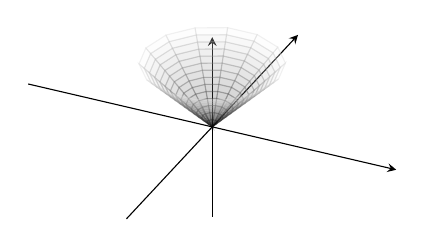
\begin{tikzpicture}
    \begin{axis}[
            axis equal,
            axis x line=center,
            axis y line=center,
            axis z line=center,
            xtick=\empty,
            ytick=\empty,
            ztick=\empty,
            xmin=-5,
            xmax=5,
            ymin=-5,
            ymax=5,
            zmin=-5,
            zmax=5]
        \addplot3[surf,opacity=0.25,samples=15,domain=0:5,y domain=0:2*pi,colormap/blackwhite]({x*0.707*cos(deg(y))},{x*0.707*sin(deg(y))},{x*0.707});
    \end{axis}
\end{tikzpicture}
%
\end{document}